\chapter{Vývoj}
\label{chap:development}

V této kapitole je popsána celková implementace modelové hry, která byla vytvořena na základě stanovených požadavků a návrhu herního systému, popsaných v předchozích kapitolách.

Hybridní deskové hře, která je finálním produktem této práce, bylo určeno pracovní jméno \textit{Trails Through Shadows} (zkratkou \textit{TTS}). I nadále však bude zmiňována především pod názvem \textit{modelová hra}. Dále je důležité zmínit, že veškerý text, který je součástí modelové hry, je napsán v angličtině.

\section{Spolupráce}
\label{sec:collaboration}

Deskové hry, především ty hybridní, mohou být velmi komplexní a náročné na vývoj. Proto byla součástí zadání práce i spolupráce na tvorbě řešení, které bylo realizováno ve skupině čtyř studentů.

\subsection{Rozdělení práce}
\label{subsec:job_distribution}

\begin{figure}[h]
    \centering
    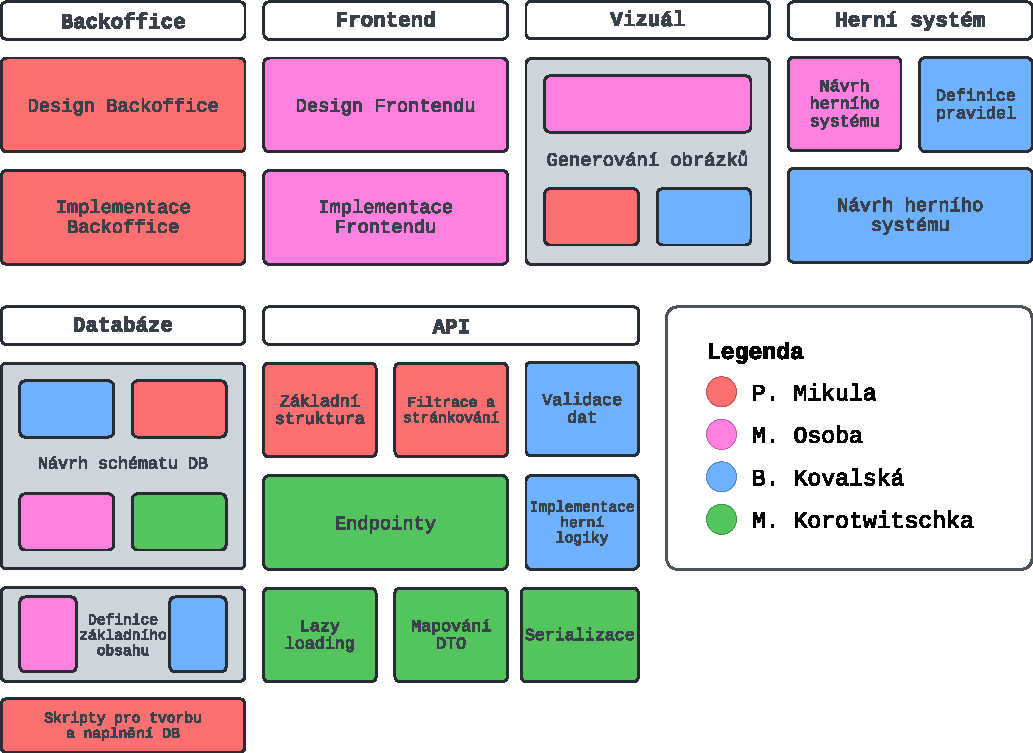
\includegraphics[width=\textwidth]{../../shared/diagrams/blocks.pdf}
    \caption{Rozložení práce v týmu}
    \label{fig:job_distribution}
\end{figure}

Hlavními čtyřmi částmi projektu byla tvorba \textbf{administrativního rozhraní} (Pavel Mikula), \textbf{uživatelského prostředí} (Miroslav Osoba), \textbf{API} (Martin Korotwitschka) a konečně implementace \textbf{herního modelu} (Barbora Kovalská), která je tématem této práce. Samotné vypracování však nebylo nutně omezeno pouze na tyto části, a tak se v průběhu vývoje mohlo stát, že se členové týmu podíleli i na jiných částech projektu.

Rozvržení práce vyobrazeno na obrázku \ref{fig:job_distribution} bylo provedeno především s ohledem na zájmy a schopnosti jednotlivých členů týmu, podle čehož se také v prvé řadě přidělovalo samotné zadání bakalářské práce. V samotném grafu byly tyto části rozděleny do bloků a rozšířeny ještě o dvě další sekce, které se ukázaly být dostatečně velké na to, aby se od ostatních osamostatnily -- \textbf{databáze} a \textbf{vizuální vzhled} hry. 

Jednotlivé bloky znázorňují určitou část dané sekce, přičemž velikost daného bloku reprezentuje mohutnost tohoto úkolu. Dílčí části, na kterých se podílelo více členů týmu, jsou reprezentovány šedě s barevnými bloky, jejichž velikost opět znázorňuje poměr práce jednotlivých spoluřešitelů.

Části projektu, na kterých se pracovalo v této práci, budou popsány v následujících sekcích.

\subsection{Organizace projektu}
\label{subsec:versioning}

\begin{figure}[h]
    \centering
    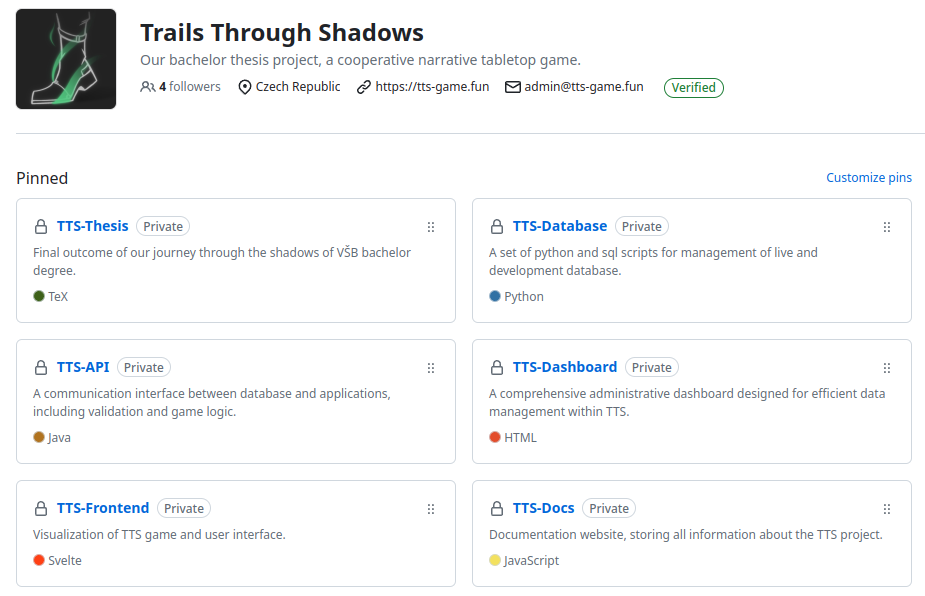
\includegraphics[width=\textwidth]{../../shared/figures/gitOrg.png}
    \caption{Rozdělení repozitářů v rámci organizace}
    \label{fig:git_organization}
\end{figure}

Pro ucelení vývoje a zajištění efektivní spolupráce byla v rámci implementace vytvořena organizace \textit{Trails Through Shadows} na platformě \textit{GitHub}\footnote{\href{https://github.com}{https://github.com}}, kde byly vytvořeny repozitáře pro jednotlivé části projektu, jak je možné vidět na obrázku \ref{fig:git_organization}. Organizace byla opatřena logem, které bylo vytvořeno v rámci zadání práce a bylo použito i pro další potřeby týmu.

\begin{description}
    \item [TTS-Dashboard] -- Administrativní rozhraní, sloužící ke správě hry, jednotlivých lokací, nepřátel a dalších entit. Primární použití je pro vývojáře, kteří zde mohou vytvářet a upravovat herní obsah.
    \item [TTS-Frontend] -- Uživatelské prostředí, které slouží k interakci se hrou. Hráči zde mohou vidět své rozehrané kampaně a postavy a také vizualizaci celého souboje včetně herní mapy, iniciativního žebříčku a nepřátel.
    \item [TTS-Api] -- API, umožňující strukturovanou komunikaci mezi databází a jednotlivými částmi hry. Obsahuje nejen základní CRUD funkcionalitu, ale i další metody pro komunikaci, autentizaci a autorizaci, validaci vstupních dat a také implementaci samotného herního systému pro správný chod hráčského prostředí.
    \item [TTS-Database] -- Nejedná se o databázi jako takovou, neboť ta je hostována na serveru, ale o skripty pro její vytvoření a naplnění výchozích dat.
    \item [TTS-Docs] -- Dokumentace projektu, taktéž hostována na serveru, která obsahuje dokumentaci, jež je vytvářena v průběhu vývoje.
    \item [TTS-Thesis] -- Repozitář pro bakalářskou práci, který obsahuje veškeré zdrojové kódy a soubory potřebné pro vygenerování této práce. Každý z členů týmu zde má svou vlastní složku, kde se nachází zdrojové kódy \LaTeX{u} jeho dokumentu, a také je zde složka \texttt{shared}, která obsahuje společné soubory, jako jsou obrázky a diagramy týkající se sdílených částí projektu. 
\end{description}

Spolu s organizací byla také zakoupena doména \texttt{tts-game.fun}, na kterou byly nasazeny veškeré části projektu, u kterých to bylo přínosné. Kontinuální integrace byla prováděna při každém commitu do hlavní větve repozitáře, kde byl vytvořen nový build a následně byl nasazen na server. Tento systém byl zajištěn pomocí služby \textit{GitHub Actions}\footnote{\href{https://github.com/features/actions}{https://github.com/features/actions}} a umožňoval všem členům týmu vidět aktuální stav projektu a jeho vývoj.

Pro zvýšení přehlednosti a efektivity souběžného vývoje tým využíval \textit{Github Issues}\footnote{\href{https://github.com/features/issues}{https://github.com/features/issues}}, kde byly vytvářeny úkoly, které bylo možné přiřadit jednotlivým členům týmu. Co se týče větví, byl využit systém \texttt{master} - \texttt{development} - \texttt{feature}, pro úkoly tedy byla vytvořena feature branch, kde byly prováděny změny a po dokončení byl vytvořen pull request do developmentu, který byl po schválení sloučen i do hlavní větve.


\section{Implementace}
\label{sec:implementation}

Během vývoje vyvstalo několik problémů, které bylo nutné řešit. Hlavním z nich byla samotná implementace herního modelu, který byl základem celé hry, ale jak je možné vidět z diagramu \ref{fig:job_distribution}, šlo i o menší prvky, na kterých bylo třeba pracovat. Tato sekce se zaměřuje na poznatky a problémy, které byly řešeny v průběhu vývoje.

\subsection{Databáze}
\label{subsec:database}

\subsection{Vizuál hry}
\label{subsec:game_visuals}

\subsection{Implementace herní logiky}
\label{subsec:game_logic}

\subsection{Validace dat}
\label{subsec:validation}

